\chapter{Silicon Photomultipliers}
Silicon PhotoMultipliers (SiPMs) are solid state light sensors also referred to as Geiger mode Avalanche Photo-Diodes (G-APDs) or Multi Pixel Photon Counters (MPPCs). They represent an interesting alternative to the more standard PhotoMultiplier Tubes (PMTs) with specific advantages as the small size, the insensitive to magnetic fields and the low power consumption.\\

The chapter will describe the working principles of these detectors (Section \ref{sec:SiPM_work}) giving an explanation to their most important features such as single-photon sensitivity, unprecedented photon number resolving capability, high internal gain, high and tunable Photon Detection Efficiency ($PDE$) (Section \ref{sec:PDE}) and excellent time resolution.
The last section is dedicated to the most important noise sources.\\

In the next chapter we will investigate their usage as light readout sensors for the IDEA dual-readout calorimeter.

\section{Working principles}\label{sec:SiPM_work}
A SiPM is a high-density matrix (up to $10^4$ per mm$^2$) of Single-Photon Avalanche Diodes (SPADs) or Avalanche PhotoDiodes (APDs). Each SPAD, also referred to as pixels or cells, is connected to the others in parallel to a single readout output.\\

\begin{figure}
	\centering
	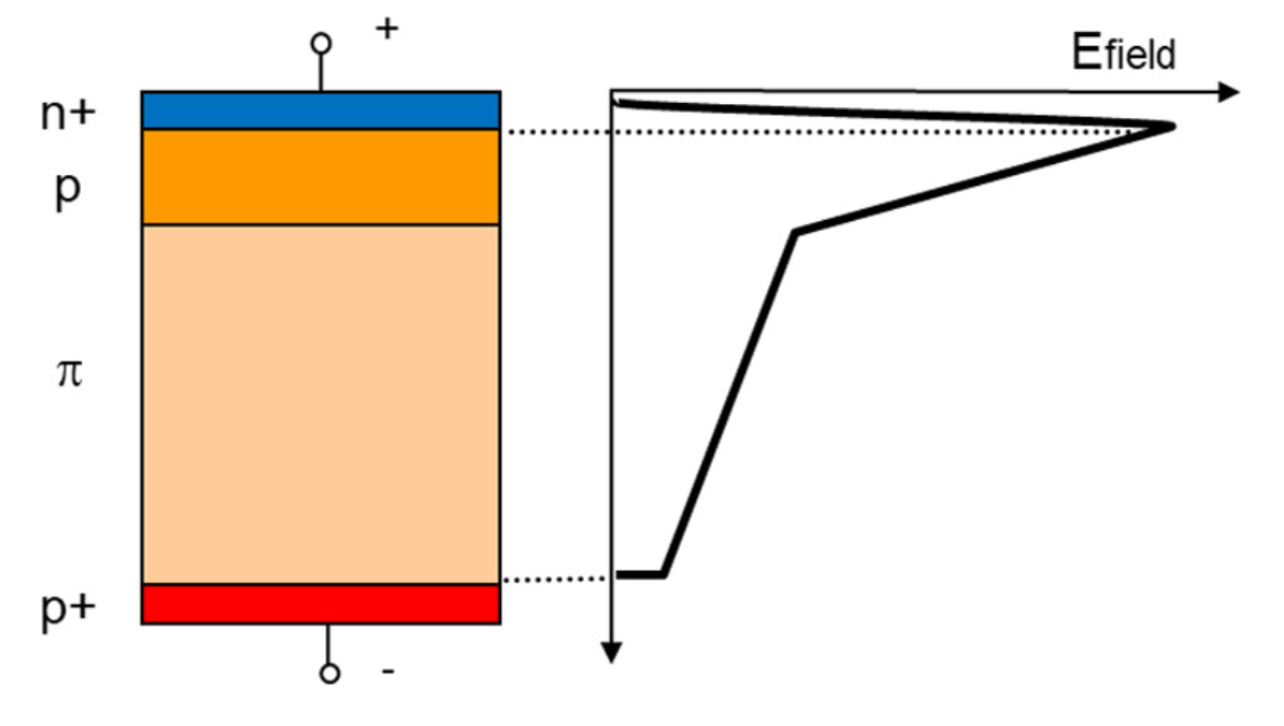
\includegraphics[width=0.8\textwidth]{IMG/Cap3/APD_struc.png}
	\caption{A sketch of a SPAD doping structure and electric field in operation mode \cite{electrics}.}
	\label{fig:APD_struc}
\end{figure}

The photodiodes are silicon elements based on the presence of an energy gap between the valence band and the conduction band of the semiconductors. In particular, they are characterized by a \textit{p-n} junction operating in the Geiger-M\"uller regime (a schematic view of the doping structure is shown in Figure \ref{fig:APD_struc}). This condition is obtained powering the APD with a few volts above the breakdown voltage ($V_{bk}$), hence, an high electric field is produced in the depletion region.
If a photon, with at least the same energy of the gap, traverses this region it can be absorbed producing charge carriers.
Operating in Geiger-M\"uller mode, the depleted region is immersed in an high electric field (tens of volts) that permits not only the collection of the carriers, but also the production of avalanche discharges. 
The peculiarity of the APDs is that the signal generated by one or more photons is indistinguishable if the photons hit the depleted region in a too short time distance. In other words, these photodetectors work as a binary device giving a signal if it is fired by at least one photon or nothing if it is not (disregarding the possibility of noise effects, see Section \ref{subsec:noise}).\\
To overcome the APDs limitations, Silicon PhotoMultipliers are composed by thousands of these small element connected in parallel as shown in Figure \ref{fig:SiPM_APD}. In this way, the SiPM can be seen as a collection of binary cells: it can provide quantitative information about the intensity of the incoming light by simply counting the number of fired cells.

\begin{figure}
	\centering
	\subfloat[]{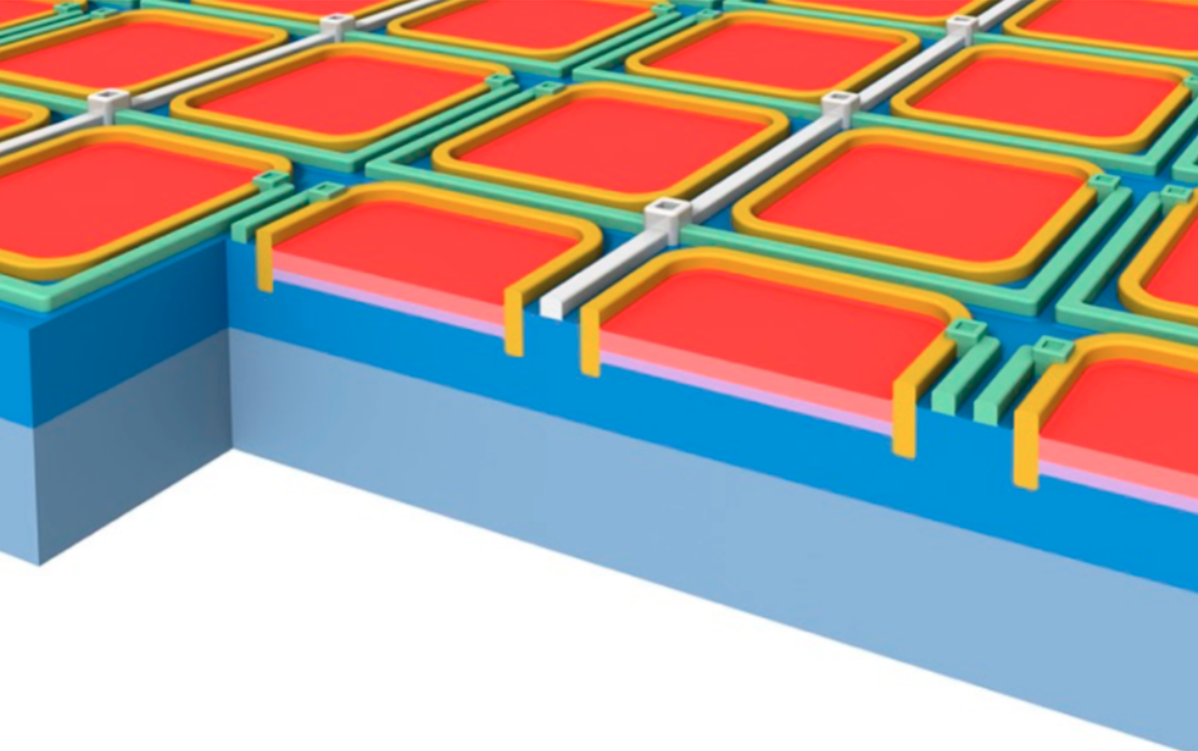
\includegraphics[height=.18\textheight]{IMG/Cap3/SiPM_APD.png}} \quad
	\subfloat[]{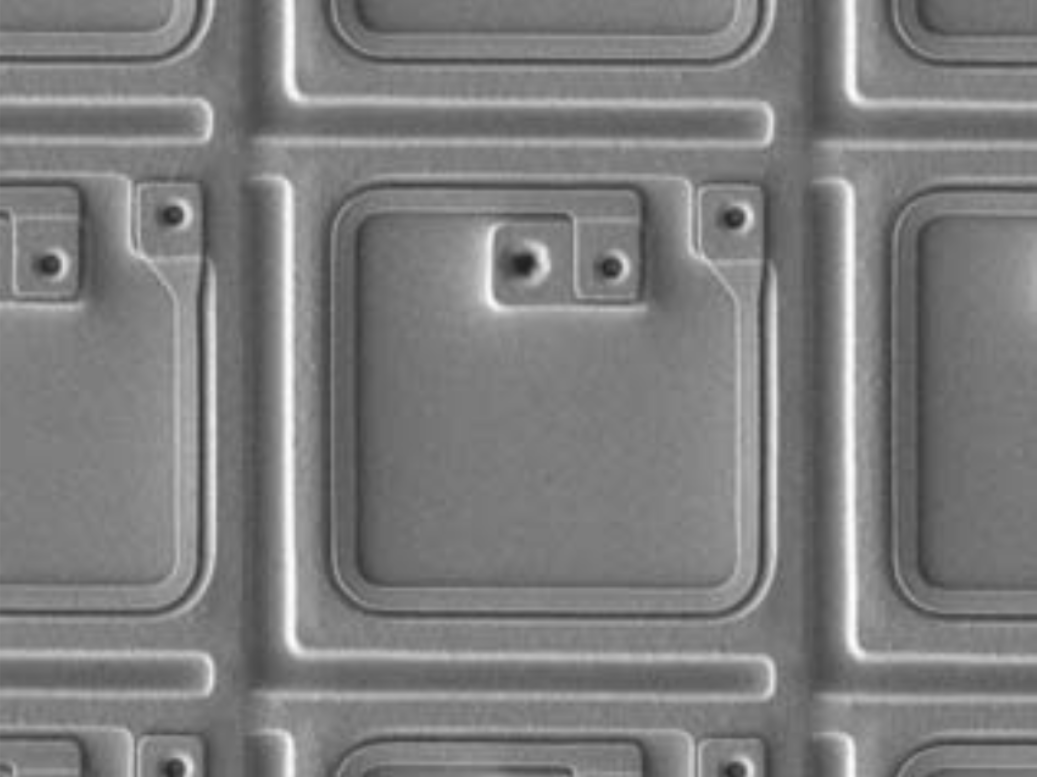
\includegraphics[height=.18\textheight]{IMG/Cap3/SiPM_APD2.png}}
	\caption{An artistic view of a SiPM structure (a). Individual  SiPM  pixels  with  metal-composite  quenching  resistor  fabricated around each cell (b). Image from \cite{SiPM_img_APD}.}
	\label{fig:SiPM_APD}
\end{figure}

\subsection*{Electrical model}
The behaviour of a single APD detector is emulated by a commonly accepted electrical model. Developed in the sixties by McIntyre and Haitz, it is sketched in Figure \ref{fig:APD_model}.\\

The detector can be interpreted as a depleted region capacitance ($C_D$) connected in parallel to a space-charge resistance ($R_S$) and a switch representing the digital avalanche product phenomenon. The Single Photon Avalanche Detector is directly connected to a quenching resistor ($R_Q$), essential to stop the high current produced by the discharge. The photon detection process start with a stationary situation where the capacitance is charged with the voltage $V_{bias}$ and the switch is set in the OFF position.\\
When a photon impinge the APD, it can produce an avalanche with a certain probability (see $PDE$ in Section \ref{sec:PDE}). The production of a discharge corresponds to setting the switch in its ON position. The consequence is the discharge of the capacitance through the internal resistance $R_S$, to the voltage $V_{BR}$ (that is lower than the bias voltage: $V_{bias} = V_{BR} + V_{ov}$) with the time constant $\tau_D \simeq R_S C_D$ \cite{electrics}. In this phase the external current increases as:
\begin{equation}
    I_{EXT}(t) = \frac{V_{ov}}{R_S + R_Q}\left( 1 - e^{-t/\tau_D} \right).
\end{equation}
At the end of the avalanche process, the switch comes back to the OFF condition and the capacitor start to recharge until the voltage $V_{bias}$. 
The recharge is characterised by a time constant called cell recovery time $\tau_R \simeq C_D R_Q$. The extern current goes to zero as:
\begin{equation}
    I_{EXT}(t) = \frac{V_{ov}}{R_S + R_Q}e^{-t/\tau_R}.
\end{equation}
The two time constant are generally different with $\tau_R \gg \tau_D$ because $R_Q$ and $R_S$ differ up to two orders of magnitude.\\
At the end of this process the APD is able to detect a new photon.\\

\begin{figure}
	\centering
	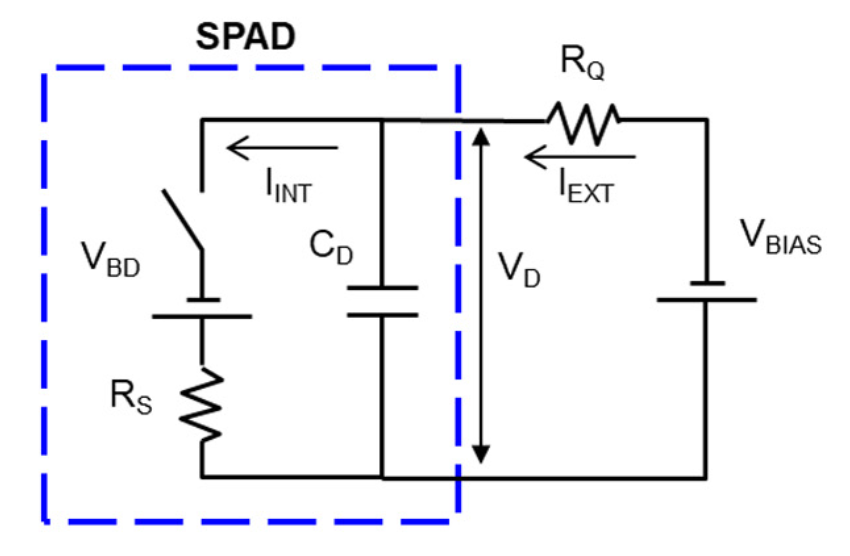
\includegraphics[width=0.8\textwidth]{IMG/Cap3/APD_model.png}
	\caption{Sketch of the equivalent circuit of a single Geiger APD \cite{electrics}.}
	\label{fig:APD_model}
\end{figure}

The conceptual output pulse produced by a single fired APD is sketched in Figure \ref{fig:wave_example}. Several APDs connected in parallel originate the signal of the whole SiPM. In the next chapter, simulated waveforms from SiPMs will be shown.\\

\begin{figure}
	\centering
	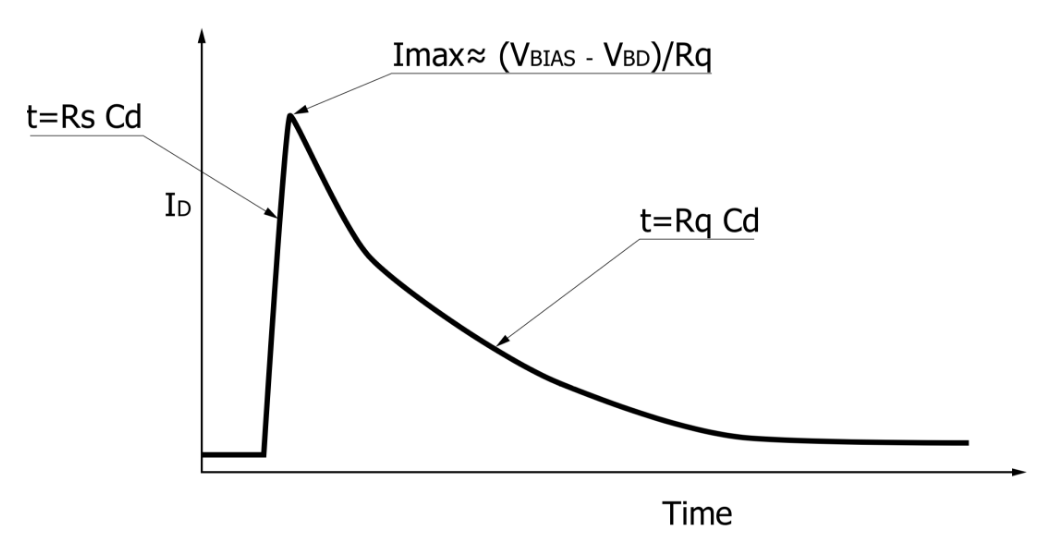
\includegraphics[width=0.8\textwidth]{IMG/Cap3/wave_example.png}
	\caption{Sketch of the conceptual output pulse produced by a single APD \cite{SiPM_img_APD}.}
	\label{fig:wave_example}
\end{figure}

\subsection*{Gain and amplitude}
The gain of a single APD is defined as the output charge in unit of elementary charge. This is a well defined quantity knowing the overvoltage and the internal capacitance:
\begin{equation}
    G = \frac{C_D V_{ov}}{q_e}.
\end{equation}
Considering a typical values as $V_{ov} \simeq 3-5$ V and $C_D \simeq 10$ fF, we obtain the standard values of $G$ of the $10^6$ order. 
Therefore, the SiPMs single photon sensitivity is well explained by this single-cell high gain.\\
A common way to evaluate the gain of a SiPM is to analyse the multi-photon charge spectrum, an example is shown in Figure \ref{fig:MPCS}.
It represent the integrated signal of a SiPM when fired with different number of photons in each event. The histogram is populated with the output charge obtained integrating the signal over a fixed time window.
Each peak is associated to events with the same number of fired cells, and, thanks to the high gain, the noise is small compared to the signal intensity. This feature permit to separate different peaks and, hence, correctly identify the number of photons detected.\\
Moreover, the distance between two consecutive peaks, expressed in unit of charge, can be used to estimate the gain via the relation $\Delta_{pp} = q_e \cdot G$ giving a direct way to evaluate the SiPM gain.\\
The number of fired cells ($N_{FC}$) follows the Poisson statistic, giving an increasing spread of the peaks that is proportional to $\sqrt{N_{FC}}$. This behaviour set a maximum number of resolvable peaks limiting the photon detection capability of these detectors.

\begin{figure}
	\centering
	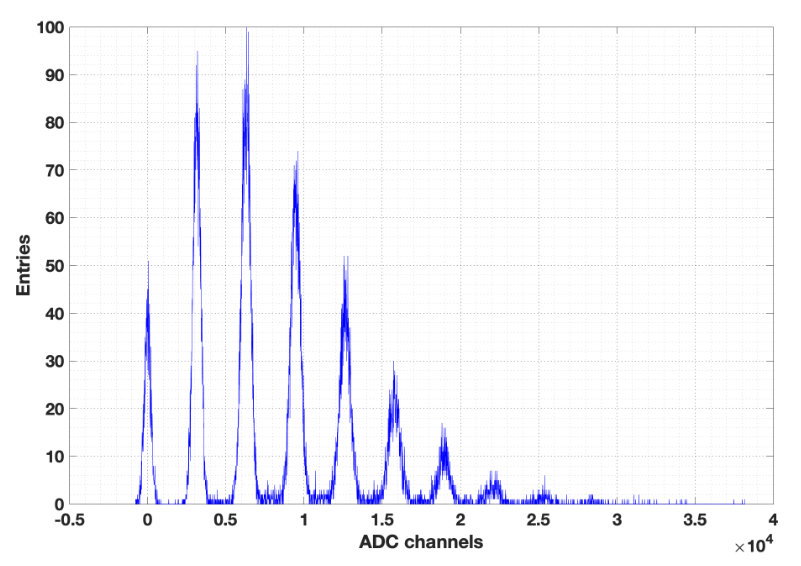
\includegraphics[width=0.8\textwidth]{IMG/Cap3/MPCS.png}
	\caption{Response of Hamamatsu MPPC 13360-1350CS illuminated by a LED: the integrated and digitized signal \cite{MPCS}.}
	\label{fig:MPCS}
\end{figure}

\section{SiPM photon detection efficiency}\label{sec:PDE}
The efficiency of a SiPM in detecting light is one of the most important parameters that characterise the detector. To numerically evaluate this feature the Photon Detection Efficiency ($PDE$) quantity has been introduced. It represent the probability of producing a signal by the SiPM when it is fired by a photon and it is quantified as the ratio of the number of fired cells that generate a signal ($N_{FC}$) and the total number of photons hitting the detector $N_{\gamma}$ \cite{PDE}.\\
The silicon light absorption coefficient is highly dependent on the wavelength of the particle, it can vary by several order of magnitude with light from UV to infrared (IR). For this reason the $PDE$ is a function of the wavelength $\lambda$ of the impinging photon, of the temperature $T$ and of the overvoltage $V_{ov}$. The $PDE$ can be written as:
\begin{equation}
    PDE = \frac{\expval{N_{FC}}}{\expval{N_{\gamma}}} = FF \times QE(\lambda) \times P_T(\lambda,V_{ov},T)
\end{equation}
where $FF$ is the geometrical fill factor, $QE$ is the quantum efficiency and $P_T$ is the avalanche breakdown triggering probability.\\
In Figure \ref{fig:PDE} a sketch of the effect of each component is shown. The $PDE$ is plotted as a function of the wavelength starting from the ideal maximal value of $1$, then is reduced by a constant contribution coming from the geometrical fill factor, then the quantum efficiency reduces it in different ways depending on the $\lambda$ and finally the trigger probability is involved with his triple dependence on wavelength, temperature and overvoltage.

\begin{figure}
	\centering
	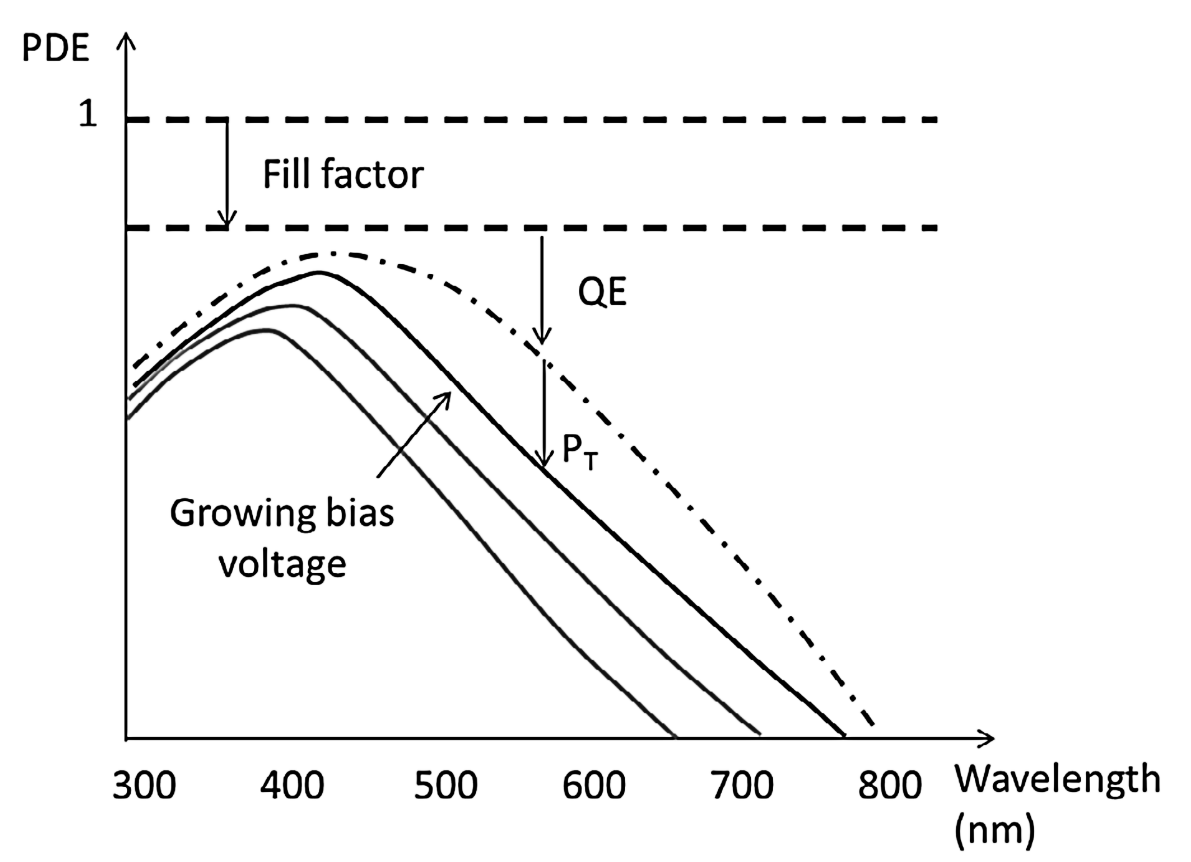
\includegraphics[width=0.8\textwidth]{IMG/Cap3/PDE.png}
	\caption{Sketch of the PDE on a blue sensitive device \cite{electrics}.}
	\label{fig:PDE}
\end{figure}

\subsection*{Geometrical fill factor}
The geometrical fill factor represents the probability that a photon impinging the SiPM traverses the active region. Quantitatively it is defined as the ratio between the sensitive area and the total area of the detector. In practical terms, the composition of SPADs also includes three main inactive regions: the guard ring, which surround each cell to quickly decrease the electric field at the border, the isolation structure between the SPADs in a SiPM needed to provide electrical and optical separation and electrical elements (i.e. quenching resistors and bias lines). 
These dead regions contribute in reducing the fill factor.\\
To minimise the dead regions area a common technique is trench isolation, it consist in a narrow depleted region placed around the active area confined with a dielectric layer. The trenches and the guard rings are typically designed together to maximise the geometrical fill factor.\\
With modern technologies the $FF$ value ranges from $90\%$ for $100$ $\mu$m down to $30\%$ for $10$ $\mu$m pixel pitch.

\subsection*{Quantum efficiency}
The quantum efficiency is the probability that an impinging photon crosses the anti-reflective coating layer and generates a pair of carriers.
The coating is a stack of different dielectric layers placed on top of the SiPM, there is not a general rule to chose the optimal layers because each application has different needs depending on the wavelength to be absorbed.\\
On the other hand, the probability to produce a $e-h$ pair by a photon highly depends on the absorption depth in the silicon. In particular, the closer to the junction the photon is absorbed, the higher the probability to produce a pair of carrier.
The absorption depth, in turn, is a function of the wavelength of the photon in such a way that it ranges from $\simeq 10$ nm for ultraviolet light up to tens of $\mu$m for infrared light.\\
The wavelength dependence can make it necessary to use particular coating called \textit{wavelength shifter}, converting photons in other photons with different $\lambda$. This process can increase the quantum efficiency and, therefore, the total $PDE$.

\subsection*{Avalanche breakdown trigger probability}
The avalanche breakdown trigger probability represent the probability of a carrier to produce an avalanche while traversing the cell high-field region. At the production of a pair in the depleted region, the two carriers are affected by the electric field and start to drift in opposite direction. The total trigger probability has a contribution from both of them:
\begin{equation}
    P_T = P_e + P_h - P_e P_h,
\end{equation}
where $P_T$ is the total trigger probability, $P_e$ and $P_h$ are the trigger probability for single carriers, the last term corrects the value when both the carriers produce an avalanche. 
The electrons trigger probability, at equal condition, is more efficient with respect to the ion trigger one because of its greater (about twice higher) ionization rate.\\
These values are electric field dependent, hence they vary with the generation position and with the power up voltage.
Summarising the dependencies, the avalanche breakdown trigger probability increases with higher overvoltage and lower temperature and it is also wavelength dependent.

\subsection{Linearity and occupancy effect}\label{subsec:occupancy_teo}
In the calorimetric measurement framework, the linearity of a detector with the particle energy is one of the most important feature.
Considering that the single charge output is almost constant for each cell of the SiPM, the greatest contribution to the non-linearity of these detectors relies on their digital nature.\\
The photon detection capability of single APDs is limited to a binary response, hence, two or more impinging photons can not be distinguished if they are temporally separated for less then the cell recovery time.\\
Starting from this consideration, the SiPM response can be considered linear when the number of photons $N_{\gamma}$ multiplied by the $PDE$ is small with respect to the number of pixels ($N_{tot}$) composing the SiPM.\\
On the other hand, while $N_{\gamma} \cdot PDE$ increases the probability of having more than one photon on the same cell becomes not negligible. In this case the occupancy effect of the SiPMs produce a saturation and a non-linear response.
Considering the random nature of the variable $N_{FC}$ and introducing the number of detected photons as $N_{pe} = N_{\gamma}\cdot PDE$, the occupancy effect can be expressed through the law:
\begin{equation}
    N_{FC} = N_{tot} \left[1 - \left(1-\frac{1}{N_{tot}}\right)^{N_{pe}}\right].
\end{equation}
The formula relates the number of fired cells $N_{FC}$ with the total number of cells $N_{tot}$ and the number of photoelectrons $N_{pe}$.
In a regime of high incident light ($N_{pe}\rightarrow \infty$), since the value $N_{tot}$ is usually greater than $100$, it can be expressed as:
\begin{equation}\label{eq:sat}
    N_{FC} = N_{tot} \left(1 - e^{-\frac{N_{pe}}{N_{tot}}}\right).
\end{equation}
We will use Equation \ref{eq:sat} when studying the linearity of a SiPM-based readout for the IDEA dual-readout calorimeter.\\
It is important to keep in mind that this formula is an approximation: it is based on the assumptions of cells uniformly irradiated, no Optical Cross-Talk, no pulse recovery effect.\\
However, considering the complicated construction of a physical model, it represent a good compromise. This statement is also supported by experimental data such as the ones produced by Hamamatsu and shown in Figure \ref{fig:occupancy}, where the fired cells are plotted as function of the $N_{\gamma}$.

\begin{figure}
	\centering
	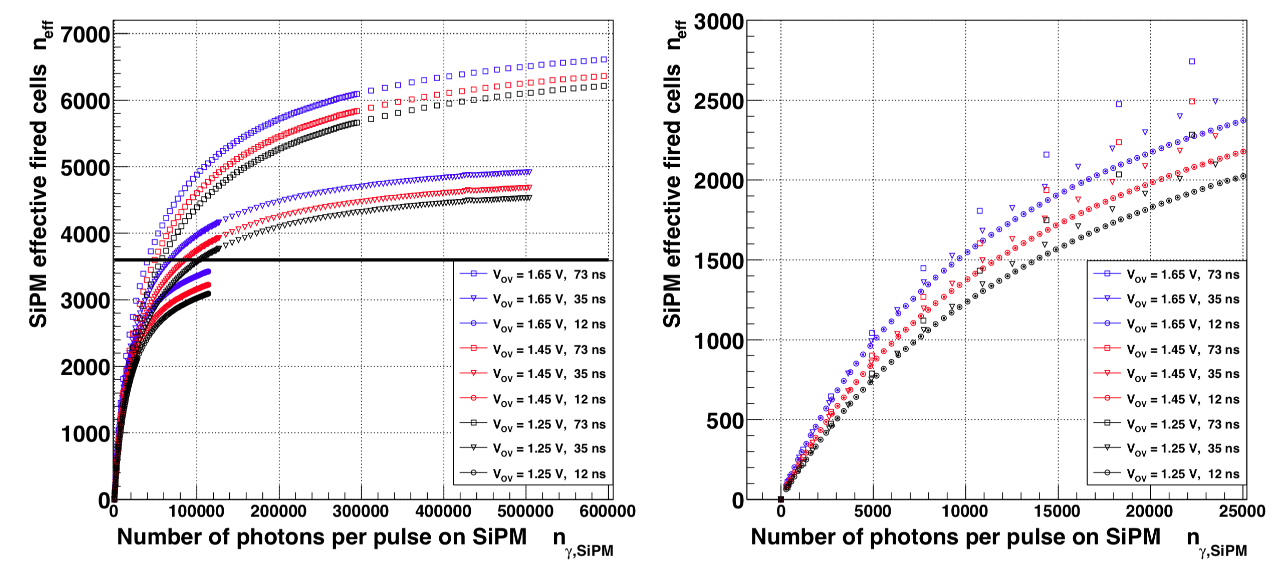
\includegraphics[width=0.95\textwidth]{IMG/Cap3/occupancy.png}
	\caption{Effective fired cells as a function of the number of photons per pulse on the active SiPM surface (full and zoom) for Hamamatsu S10362-050C type, $250$ ns gate length \cite{occupancy}.}
	\label{fig:occupancy}
\end{figure}

\section{Noise effects}\label{subsec:noise}
When a SiPM is powered up, at least three noise sources are present and must be known \cite{electrics}.\\
Noises can be distinguished in two categories: primary noise and correlated noise. Primary noises arise when a carrier, generated through thermal generation or tunneling, traverse the depleted region of a SPAD and trigger the Geiger avalanche.\\
On the other hand, a correlated noise is identified as an avalanche discharge triggered by another previous signal in the SiPM.
A sketch of the most important noises that effect SiPM is shown in Figure \ref{fig:sipm_noises}.

\begin{figure}
	\centering
	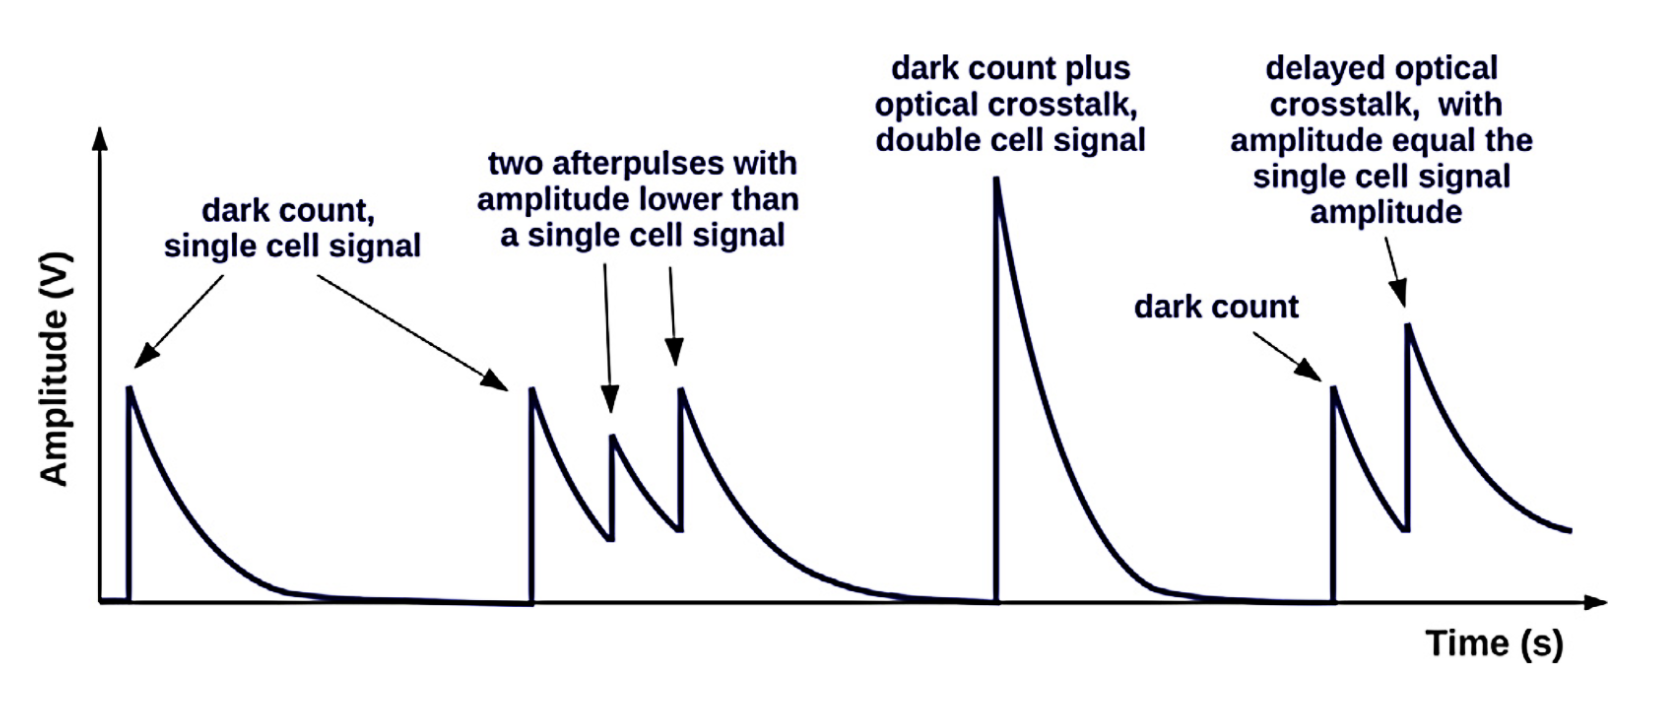
\includegraphics[width=0.9\textwidth]{IMG/Cap3/sipm_noises.png}
	\caption{Sketch of the different SiPM output noise signals \cite{APD_new_ph}.}
	\label{fig:sipm_noises}
\end{figure}

\subsection{Dark Count Rate}
In the depleted region, the generation of free carrier is possible also in absence of light. These type of signals are called \textit{dark counts} and are associated to the numerical value of the Dark Count Rate (DCR). With modern technologies the DCR value ranges from tens of kHz to MHz per mm$^2$. Most of the electron-hole pairs are generated thermally or by the electric field, these sources produce the same pulse obtained from a photoelectron. The genesis of the signal are indistinguishable, hence, the impact of the dark count rate can be mitigate only through an average correction.\\
The thermally generated pairs can be reduced lowering the detector temperature, and the ones produced by the electric field can be reduced lowering the field itself. However this effect has a smaller impact then the thermal one.\\

\subsection{Optical Cross-Talk}
During the avalanche process, there are, on average, $3$ emitted photons every $10^5$ carrier that cross the junction with at least $1.14$ eV (the band gap of silicon). These photons can trigger an avalanche in a neighbour cell, producing a signal that is classified as correlated noise under the name of \textit{Optical Cross-Talk} (OCT).\\
The noise production process is roughly instantaneous, making impossible to separate the true signal from the noise. The effect results in a pulse doubled with respect to the correct one.\\
Considering, for example, a SiPM with a gain of $10^6$, each avalanche discharge produce on average $30$ photons that can reach neighbouring cells and trigger noise signals.
At present, to mitigate this effect, SiPM cells are surrounded by elements coated with reflective material reducing the OCT probability to $1-2\%$.\\

\subsection{After-Pulse}
Another source of correlated noise is known as \textit{afterpusing} (AP). When an avalanche discharge occurs, carriers can be trapped by impurities in the high-field region. They can be released after a delay time that can range from few ns up to several $\mu$s. Once they are released, these carrier produce a signal in the same cell where they were generated. Hence the signal is delayed and its amplitude depends on the delay time: the greater the delay time, the more the cell is recharged, the higher the produced signal amplitude.\\
In first approximation, the charge ratio between the AP and the original pulse follows the law:
\begin{equation}
    \frac{Q_{AP}}{Q} = 1 - e^{-\frac{\Delta t}{\tau_r}}
\end{equation}
where $\Delta t$ is the delay time and $\tau_r$ is the cell recovery time constant.\\
The probability of this correlated noise can be lowered reducing the overvoltage value (with the side effect of reducing the SiPM gain) or increasing the temperature (producing also an increse of DCR and OCT probabilities).\\
Using high quality silicon lattices, the afterpulse noise probability is reduced to values of $1-3\%$.\\
